\documentclass[12pt,letterpaper]{article}
\usepackage[utf8]{inputenc}
\usepackage[T1]{fontenc}
\usepackage{amsmath}
\usepackage{amssymb}
\usepackage{graphicx}
\usepackage[spanish]{babel}
\title{Portafolio Metodología de la Investigación}
\author{Arnoldo Del Toro Peña}
\usepackage{pdfpages}
\usepackage{hyperref}
\begin{document}
\section*{Tarea 1}
Investiga los requerimientos de por lo menos cinco universidades extranjeras sobre el contenido y la estructura de un anteproyecto (research proposal); incluye citas claras a tus fuentes. Acorde a tus hallazgos, prepara un esqueleto de estructura para tu propio anteproyecto.
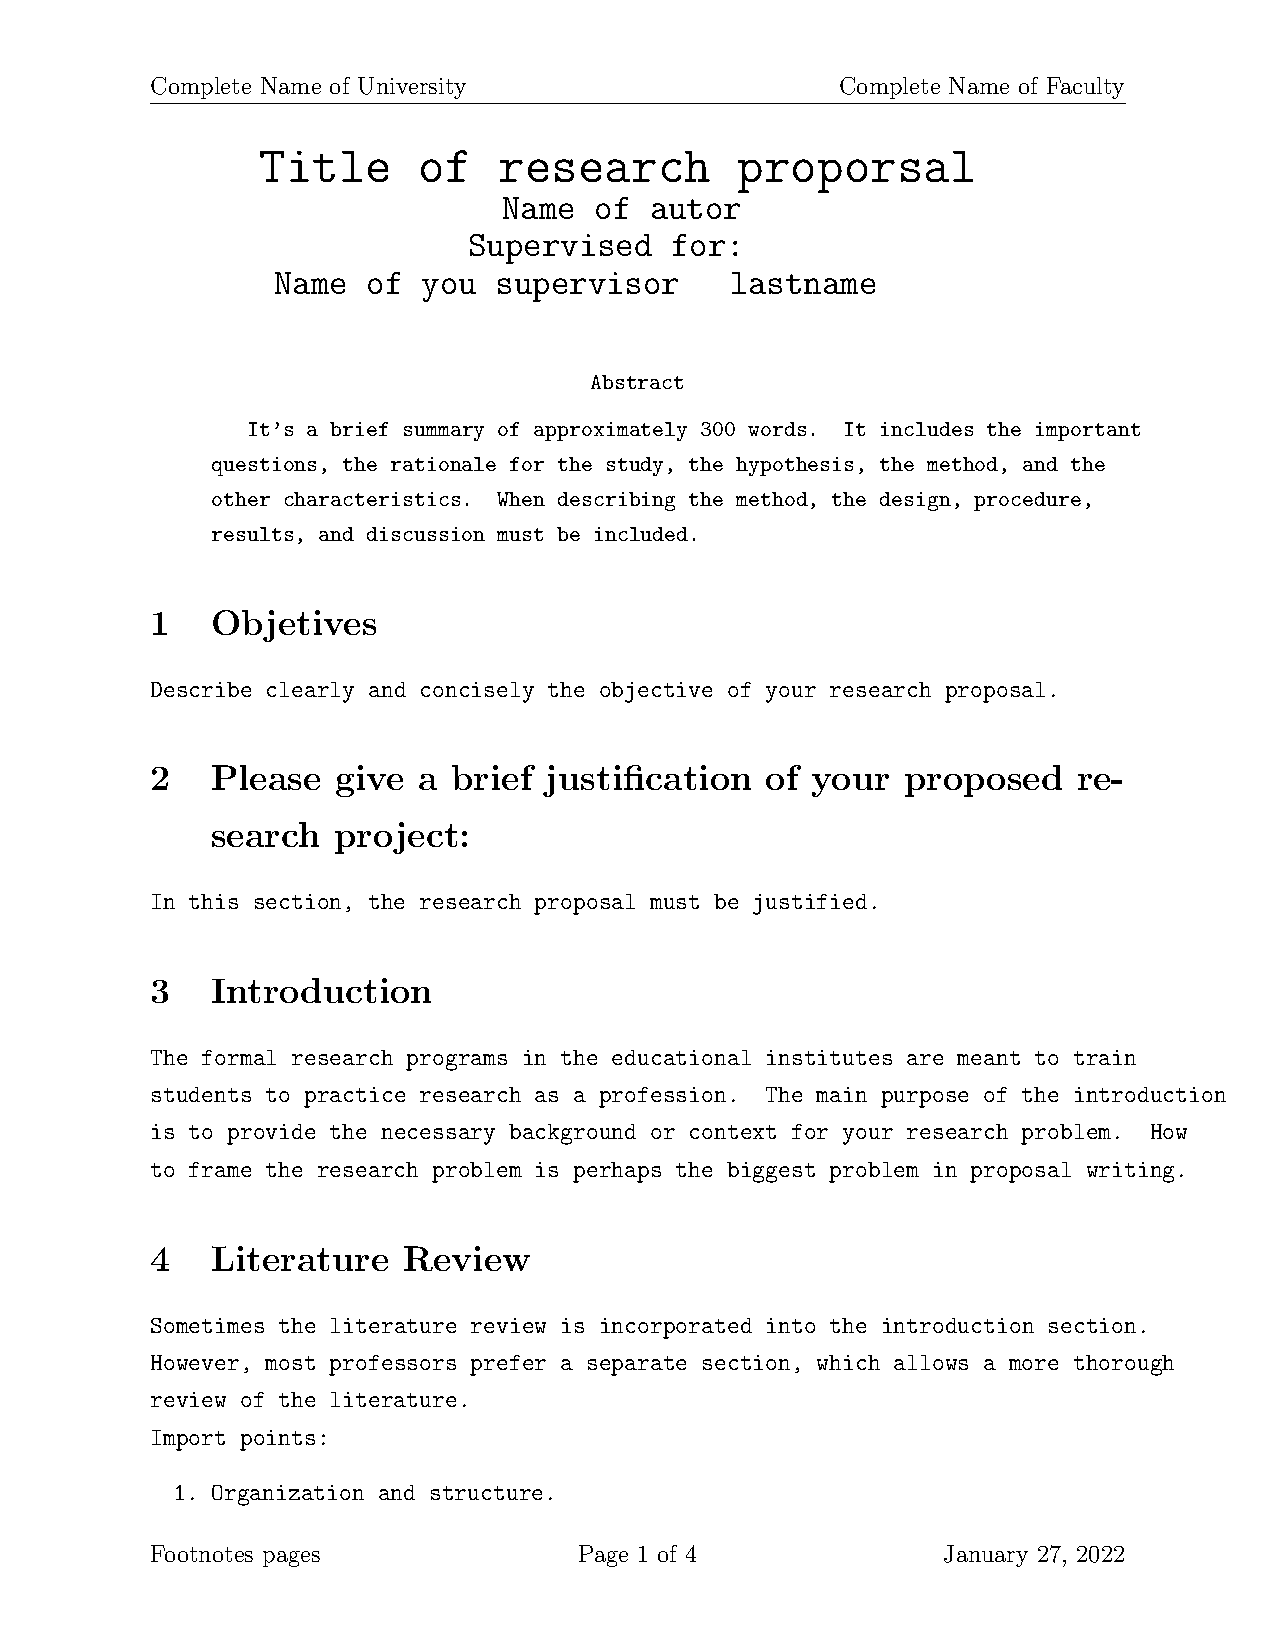
\includepdf[pages=-]{tarea1.pdf}
\section*{Tarea 2}
Investiga los requisitos y recomendaciones para secciones relacionados a reportaje de la metodología en por lo menos cinco revistas indizadas de tu área de estudio; incluye citas claras a tus fuentes. Acorde a tus hallazgos, prepara un esqueleto de estructura para la sección de metodología de tu anteproyecto.
\includepdf[pages={2,3}]{tarea2.pdf}
\section*{Tarea 3}
Redacta la sección de metodología. Recuerda incluir la bibliografía ya citada y deja el resto del documento en el estado esqueleto de antes.
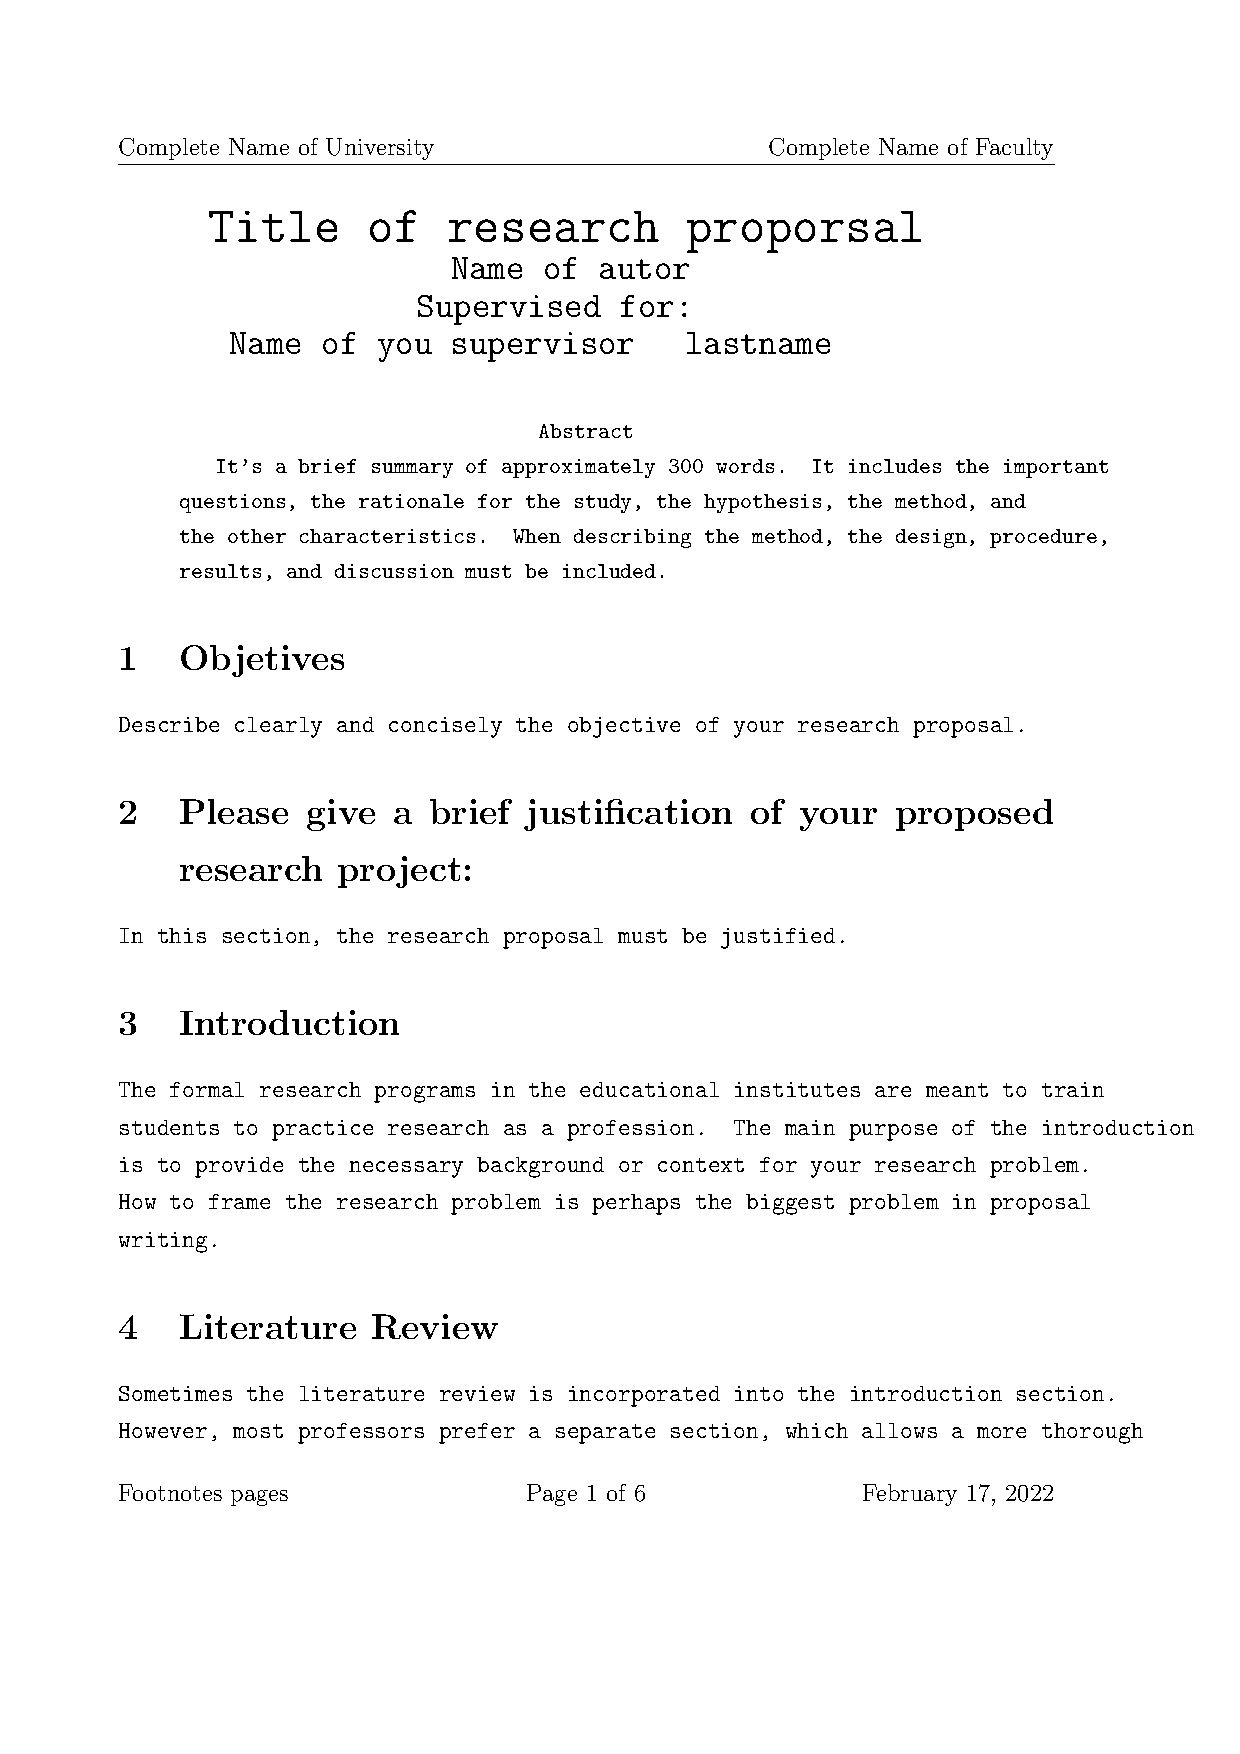
\includepdf[pages = -]{tarea3}
\section*{Tarea 4}
Investiga las guías sobre referencias de por lo menos tres revistas indizadas de tu área igual como los lineamientos bibliográficos referentes a las tesis de su nivel de por lo menos tres universidades extranjeras; incluye citas claras a tus fuentes. Acorde a tus hallazgos, analiza qué tan bien la bibliografía citada en tu borrador actual de la tesis cumple con lo solicitado.
\section*{Tarea 5}
Redacta las secciones que cubren la introducción, los antecedentes y el estado de arte de tu anteproyecto, asegurando que la bibliografía citada (siendo un subconjunto de lo que citarás en la tesis), cumple con los lineamientos que definiste en la tarea anterior.
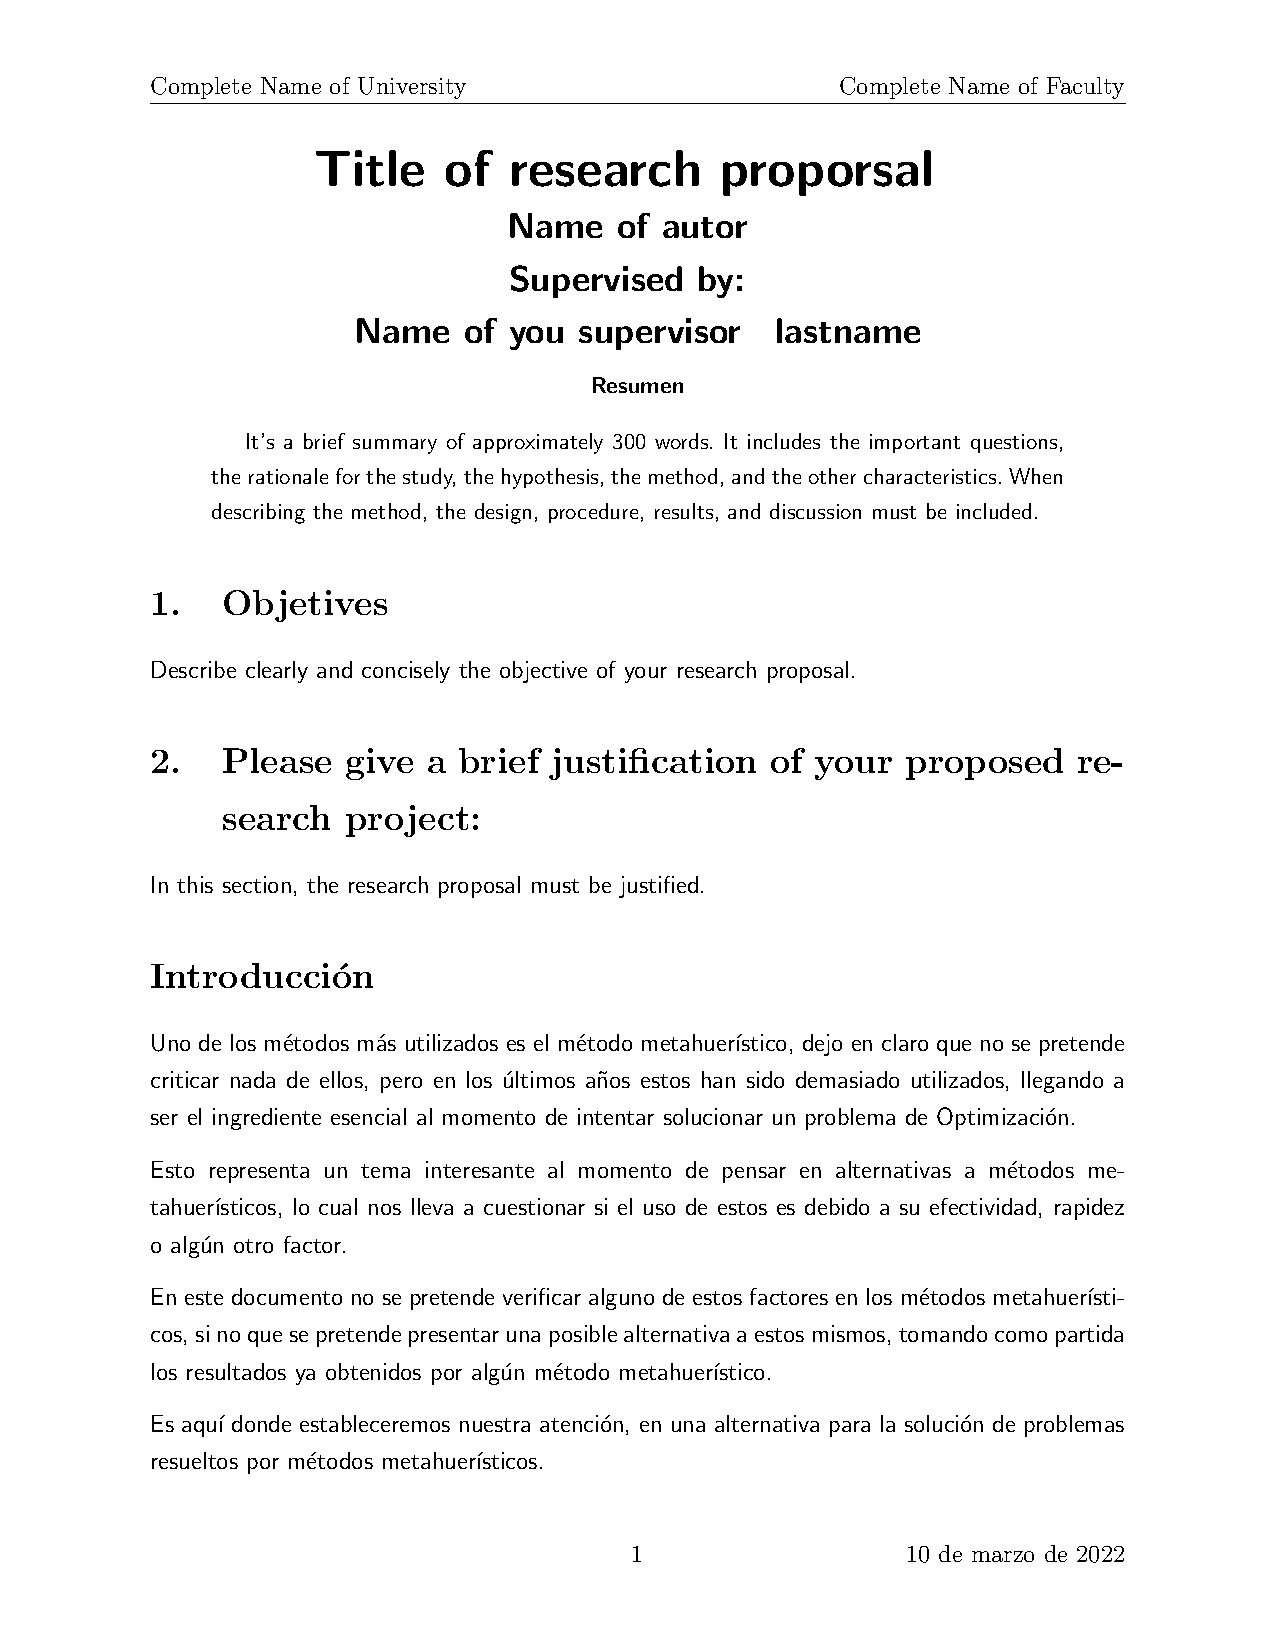
\includepdf[pages = -]{tarea45}

\section*{Tarea 6}
Investiga las indicaciones sobre el reportaje de la solución propuesta y resultados experimentales de por lo menos tres revistas indizadas de tu área y aquellas sobre tesis de su nivel de estudios de por lo menos tres universidades extranjeras; incluye citas claras a tus fuentes. Acorde a tus hallazgos, prepara un "checklist" sobre aspectos de la solución propuesta y experimentos por incluir en el anteproyecto para que cumpla con lo solicitado.
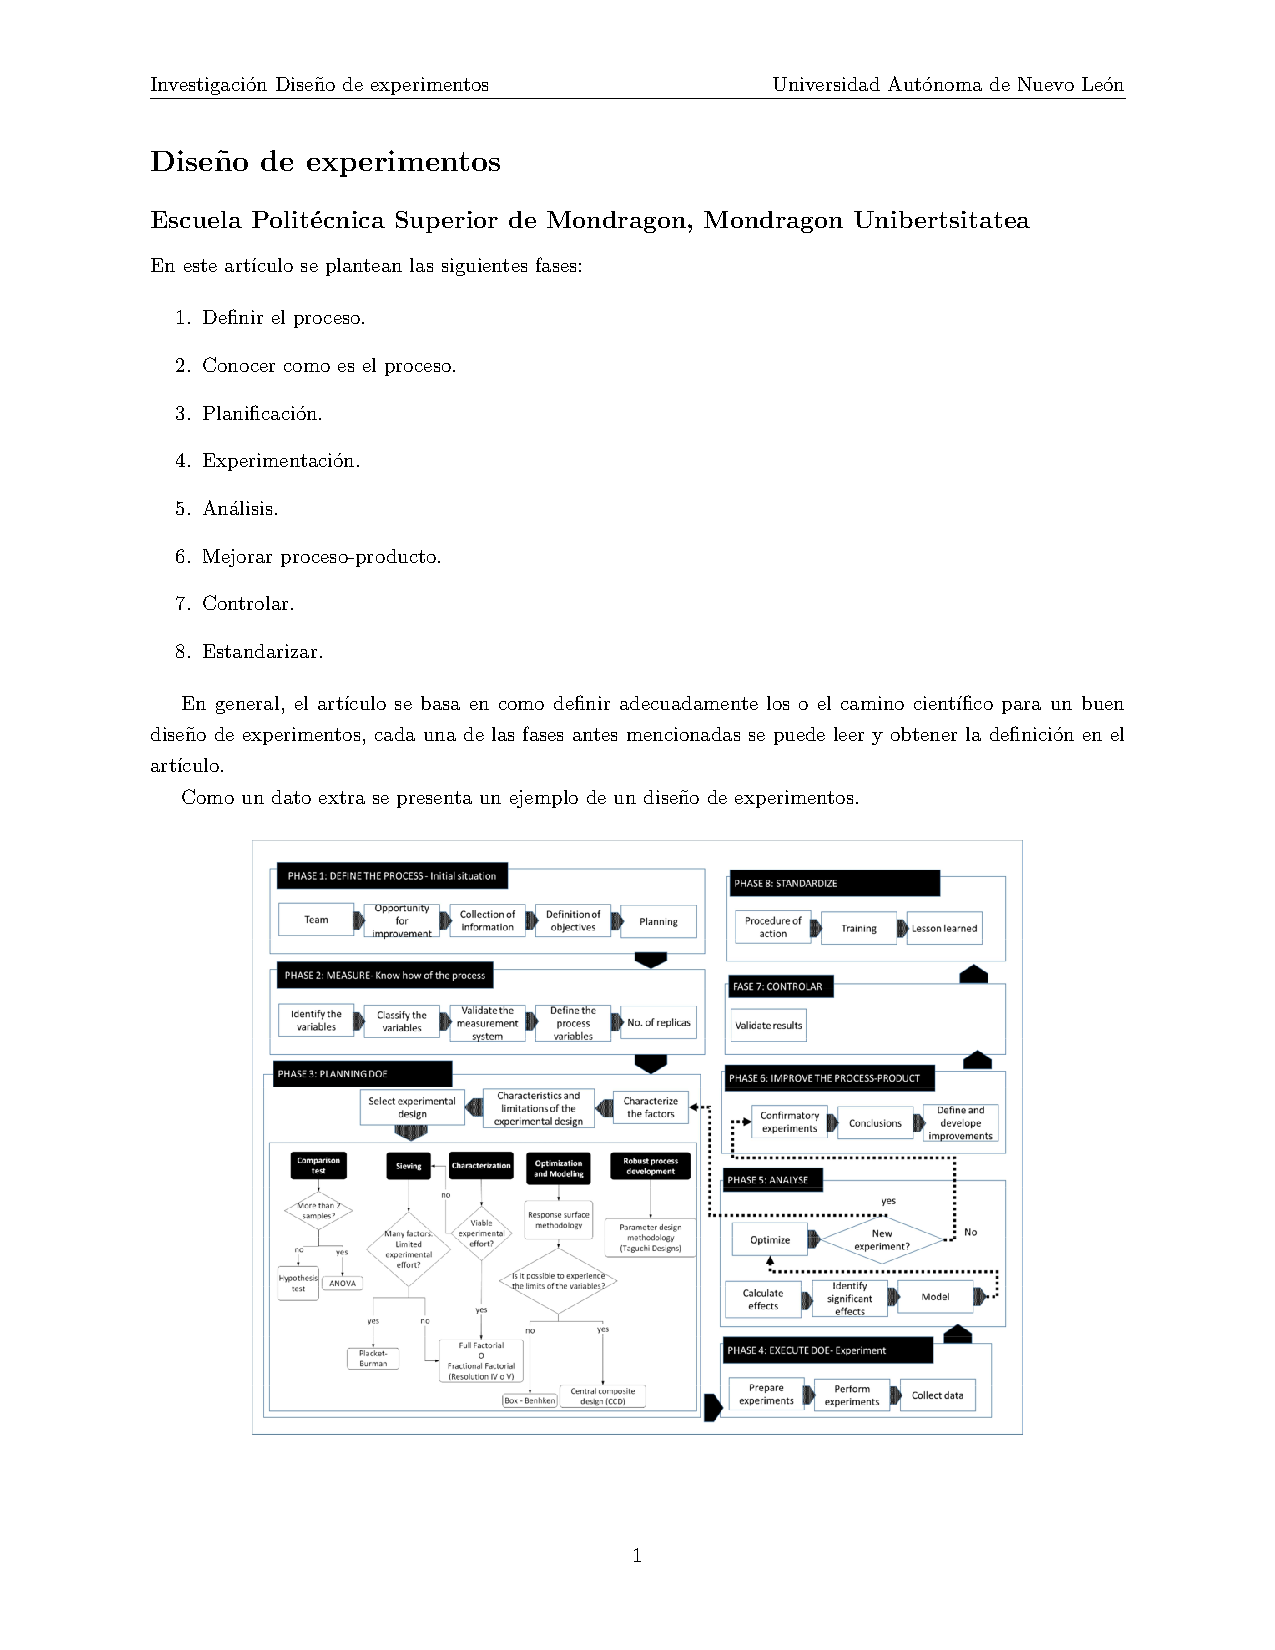
\includepdf[pages = -]{tarea6.pdf}
\section*{Tarea 7}
Redacta las secciones que cubren la solución propuesta y diseño experimental de tu anteproyecto, asegurando que la bibliografía citada (siendo un subconjunto de lo que citarás en la tesis), cumple con los lineamientos que definiste en la tarea anterior.
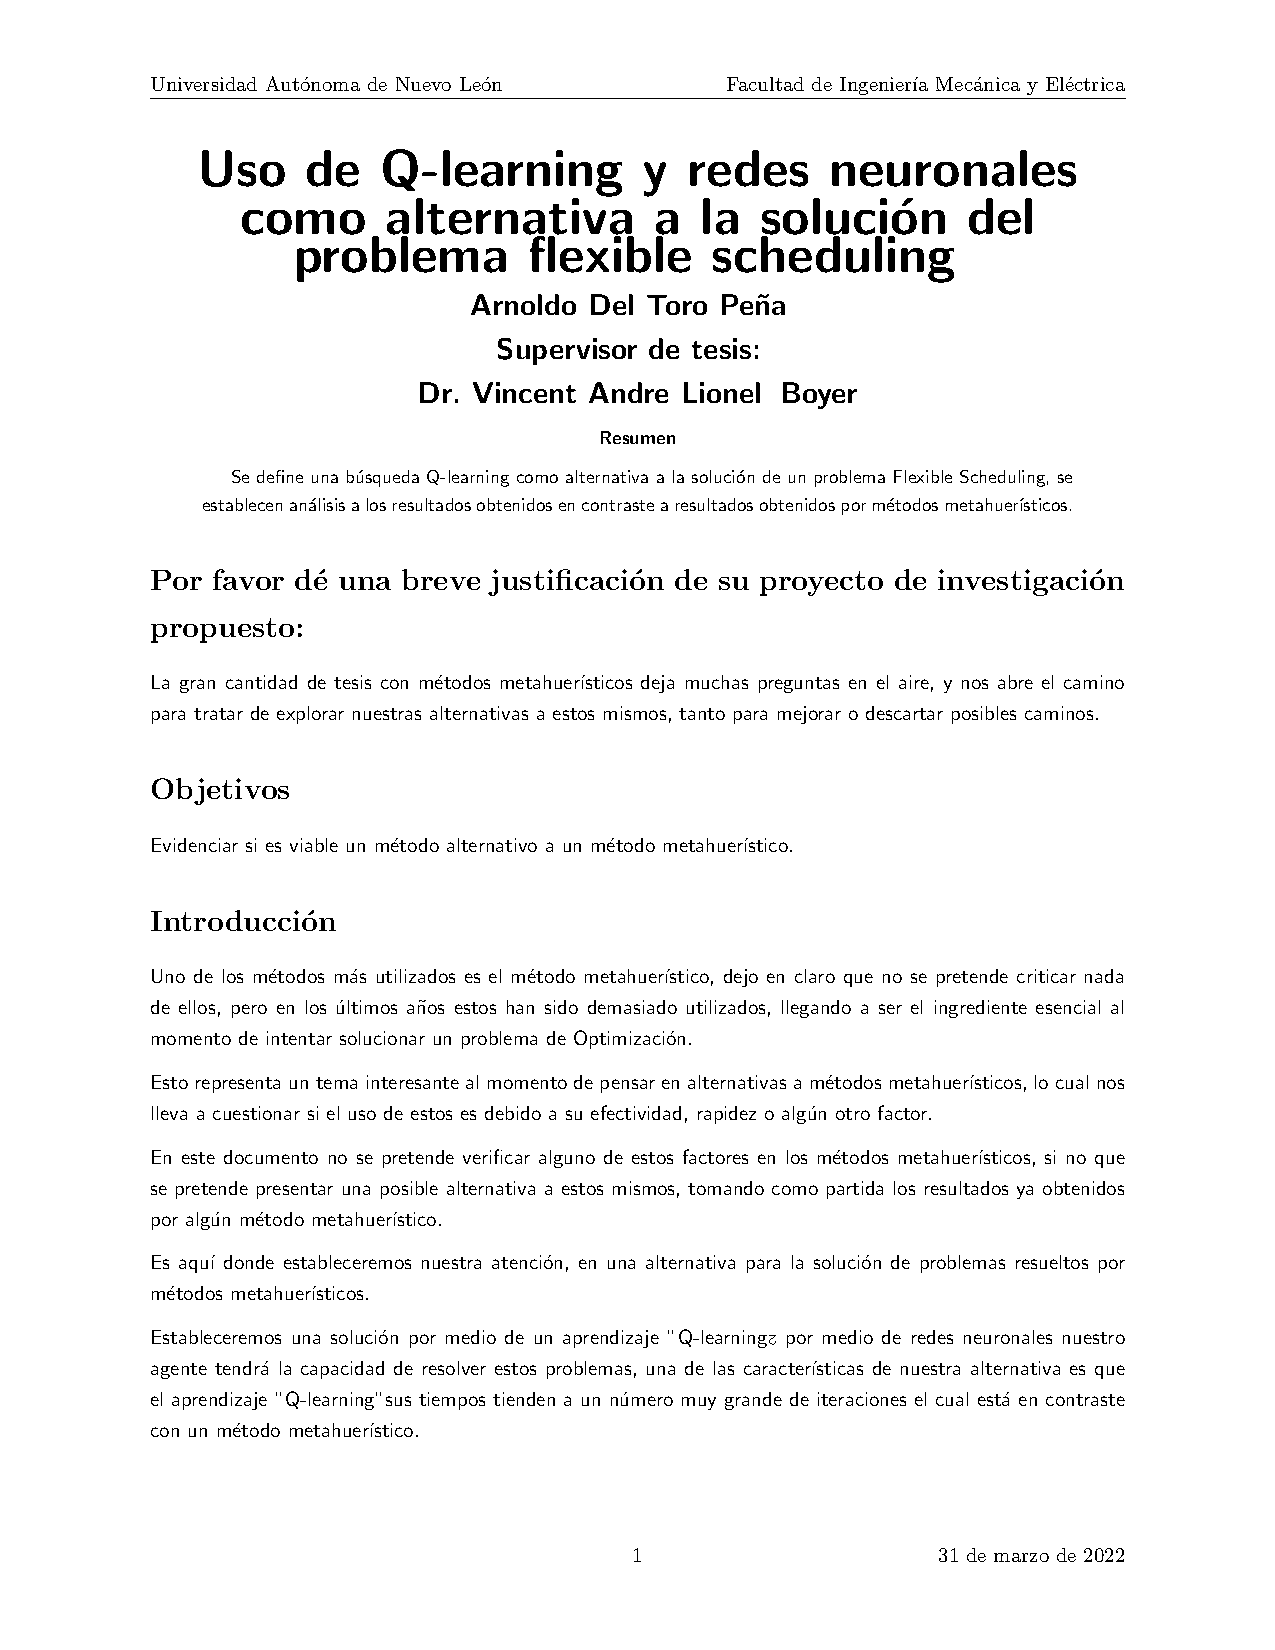
\includepdf[pages = -]{tarea7}
\subsection*{Versión final}
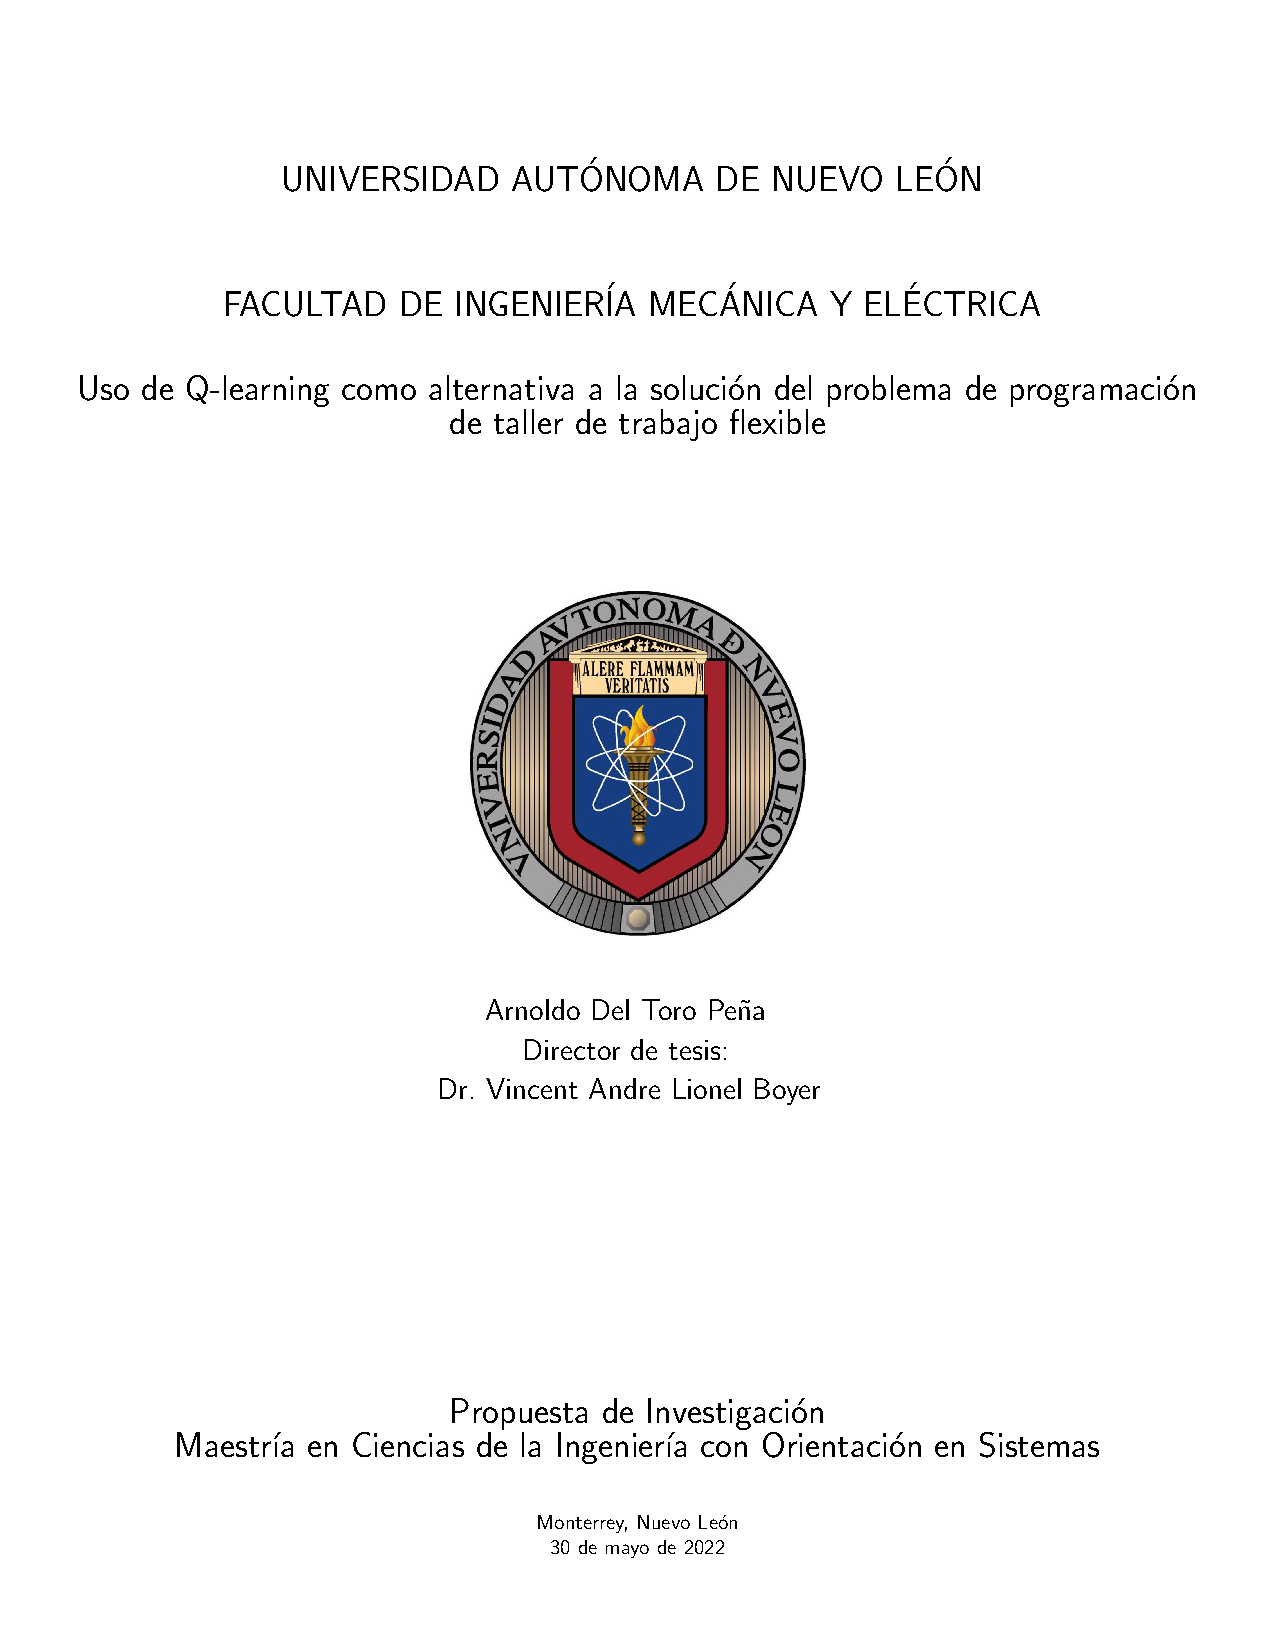
\includepdf[pages=-]{escrito-final-arnoldo-del-toro}
\section*{Tarea 8}
Crea una ID ORCID y perfiles de Scopus, Google Scholar y ResearchGate; si ya los tienes, actualizarlos. Incluyelos en tu CV junto con tu repositorio de GitHub y actualiza el CV también. Identifica y sigue a por lo menos cinco expertos de tu área en Google Scholar; revisa si tienen cuentas de Twitter y/o GitHub que puedas seguir. Evidencia todas estas actividades en tu entregable de la semana.
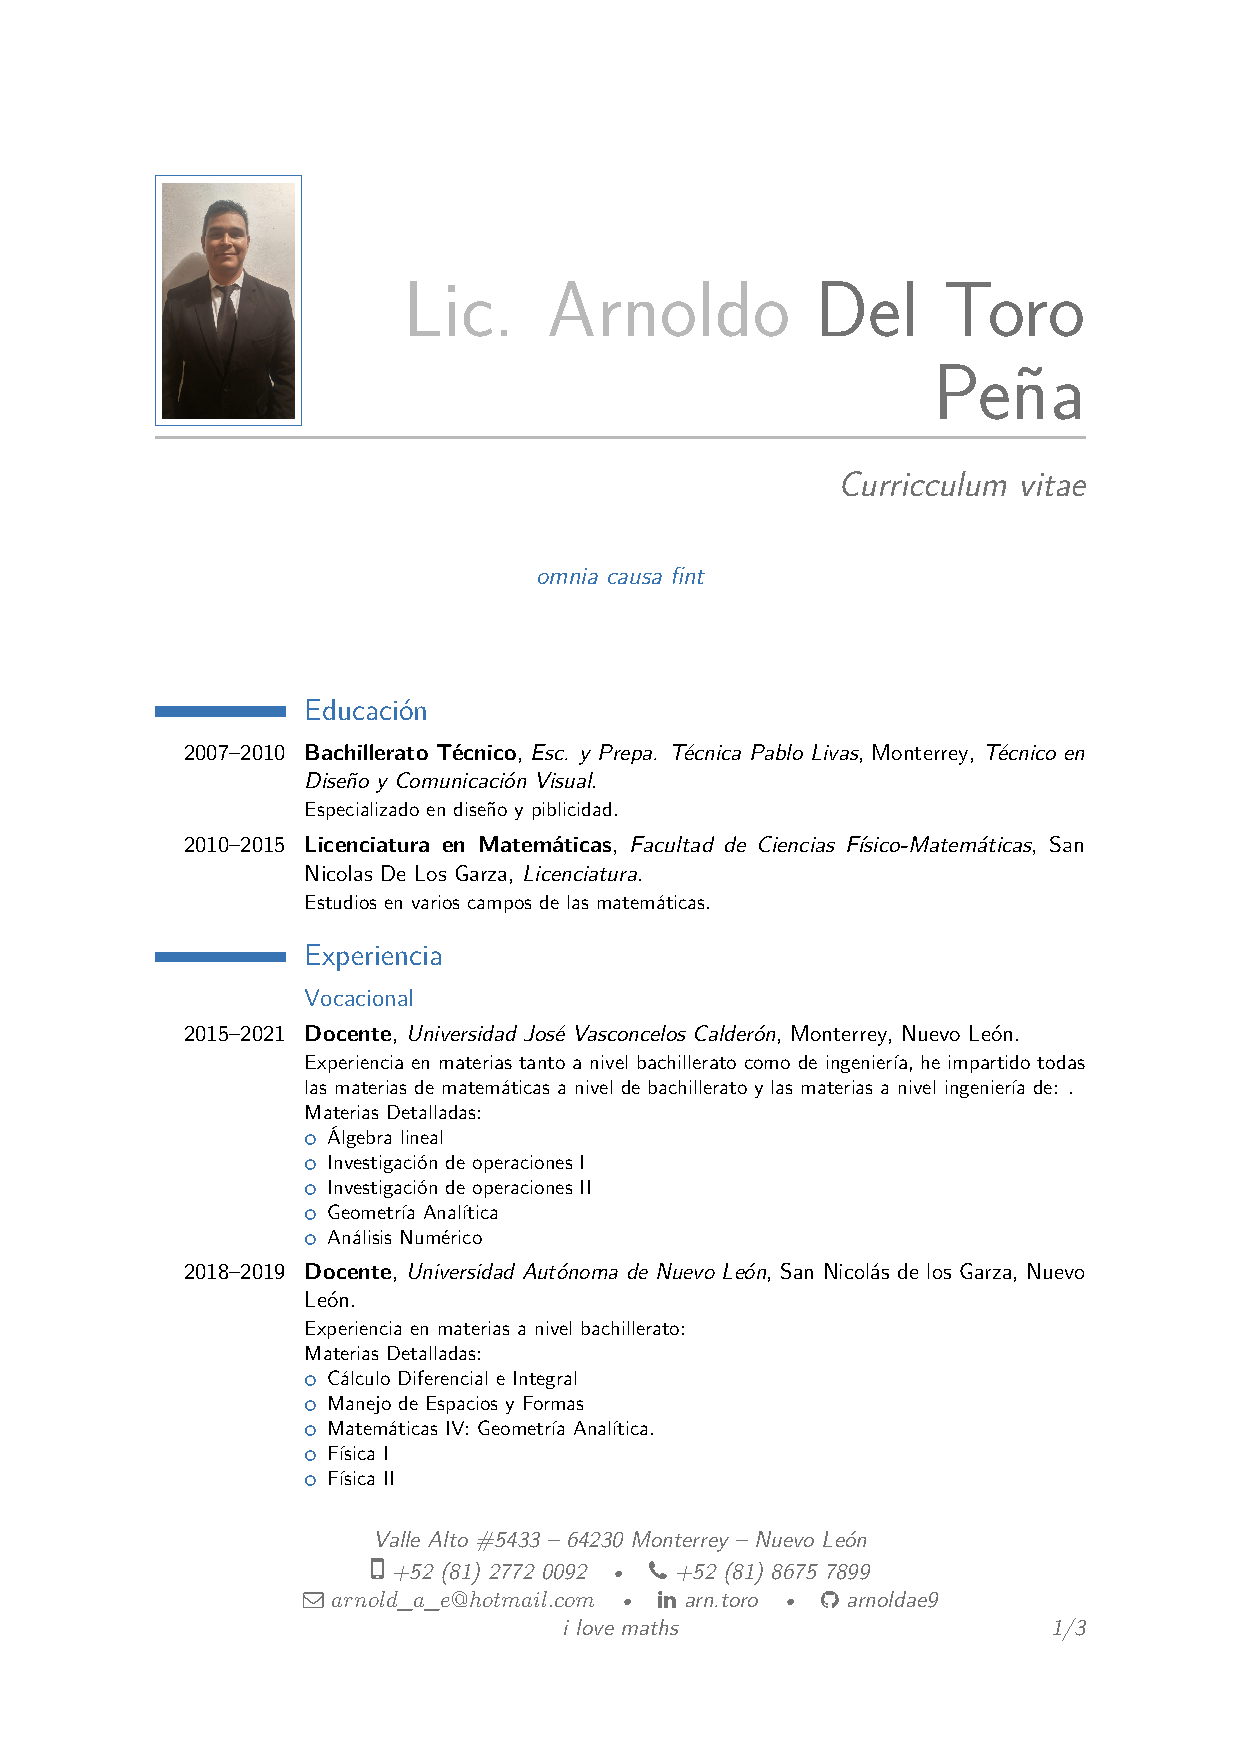
\includepdf[pages = -]{cv}
\section*{Tarea 9}
Investiga sobre repositorios de pre-prints de tu área, sobre la política de pre-prints de por lo menos tres revistas indizadas potenciales para publicar los resultados de tu proyecto. Investiga también potenciales mailing lists de tu área particular. Documenta los hallazgos en tu entregable de la semana.
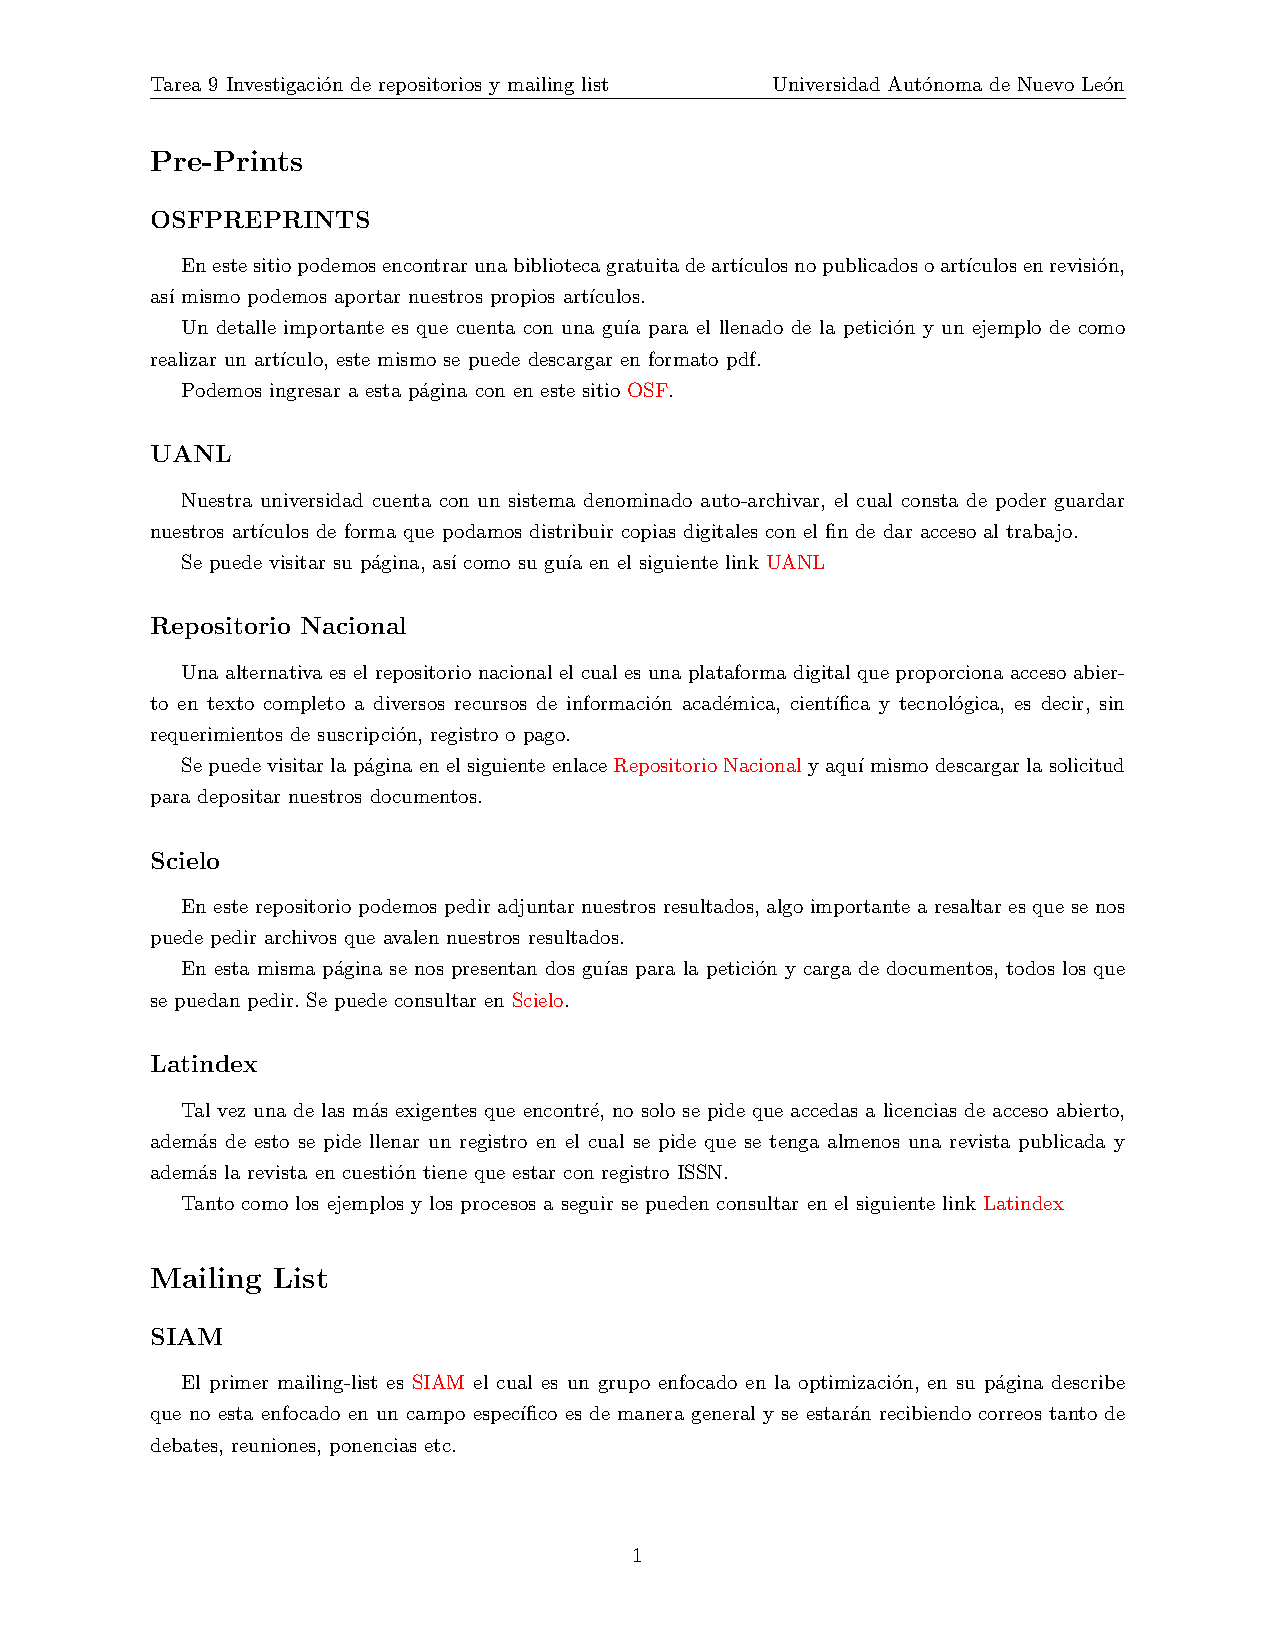
\includepdf[pages = -]{tarea9}
\section*{Tarea 10}
Prepara en LaTeX con beamer diapositivas sobre tu anteproyecto. Ensaya la presentación grabándote y toma tiempo de cuánto tardaste en presentarla. No incluyas la grabación en el entregable, pero sí un screenshot de su duración.
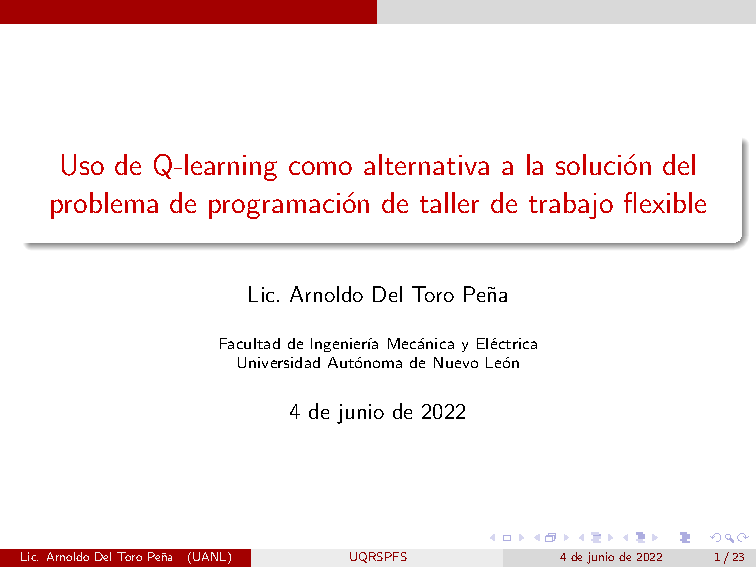
\includepdf[pages = -]{presentacion}
\section*{Comentarios}
\begin{figure}[h!]
	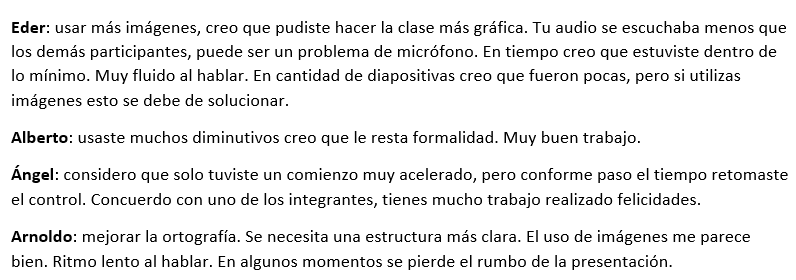
\includegraphics[scale = 0.5]{comentarios}
\end{figure}

\section*{Autoevaluación: 5 }
 Mi trabajo final no es excelente; sin embargo al ver los primeros escritos contra el resultado final el avance es indiscutible, y estoy totalmente seguro que el material y las recomendaciones que obtuve me servirán más adelante.
 
\vspace{1 cm}
Por último link de la presentación: \url{https://youtu.be/Y_Wzk6niUt0}
\end{document}